\chapter{Definition}
Der MPD ist eine Client/Server-Architektur, in der die Clients und Server (MPD ist der Server)
über ein Netzwerk interagieren. MPD ist also nur die Hälfte der Gleichung. Zur Nutzung von  
MPD, muss ein MPD-Client (auch bekannt als MPD-Schnittstelle) installiert werden.
Als Netzwerkprotokoll wird das MPD eigene Protokoll verwendet. \footnote{http://www.musicpd.org/doc/protocol/index.html}
\section{Definition des MPD}
\begin{quote}
    Der Music Player Daemon (kurz MPD) ist ein Unix-Systemdienst, der das Abspielen von Musik auf 
    einem Computer ermöglicht. Er unterscheidet sich von gewöhnlichen Musik-Abspielprogrammen dadurch, 
    dass eine strikte Trennung von Benutzeroberfläche und Programmkern vorliegt. Dadurch ist die 
    grafische Benutzeroberfläche auswechselbar und auch eine Fernsteuerung des Programms über das 
    Netzwerk möglich. Die Schnittstelle zwischen Client und Server ist dabei offen dokumentiert und 
    der Music Player Daemon selbst freie und quelloffene Software.\ \\ \\
    Der MPD kann wegen seines geringen Ressourcenverbrauchs nicht nur auf Standartrechnern sondern 
    auch auf einem abgespeckten Netzwerkgerät mit Audioausgang betrieben werden und von allen Computern
    oder auch Mobiltelefonen / PDAs im Netzwerk ferngesteuert werden.\ \\ \\
    Es ist auch möglich den Daemon und den Client zur Fernsteuerung lokal auf dem gleichen Rechner
    zu betreiben, er fungiert dann als normaler Medienspieler, der jedoch von einer Vielzahl 
    unterschiedlicher Clients angesteuert werden kann, die sich in Oberflächengestaltung und Zusatzfunktionen
    unterscheiden. Mittlerweile existierten auch zahlreiche Clients, die eine Webschnittstelle bereitstellen.\ \\ \\
    Der MPD spielt die Audioformate Ogg Vorbis, FLAC, OggFLAC, MP2, MP3, MP4/AAC, MOD, Musepack und wave ab.
    Zudem können FLAC-, OggFLAC-, MP3- und OggVorbis-HTTP-Streams abgespielt werden. Die Schnittstelle kann
    auch ohne manuelle Konfigruation mit der Zeroconf-Technik angesteuert werden. Des Weiteren wird Replay
    Gain, Gapless Playback, Crossfading und das Einlesen von Metadaten aus ID3-Tags, Vorbis comments oder
    der MP4-Metadatenstruktur unterstützt.
    \footnote{Zitat aus: http://de.wikipedia.org/wiki/Music\_Player\_Daemon}
\end{quote}
\newpage
\subsection{Der MPD kann:}
\renewcommand{\labelitemi}{•}
\begin{itemize}
    \item Musik abspielen
    \item Musik kontrollieren und in Warteschlangen reihen 
    \item Musik Dateien dekodieren
    \item HTTP-Streaming
        \renewcommand{\labelitemi}{--}
        \begin{itemize}
            \item Eine HTTP-URL kann zur Warteschlange hinzugefügt oder direkt abgespielt werden.\\
        \end{itemize}
\end{itemize}

\subsection{Der MPD kann nicht:}
\begin{itemize}
    \item Album-Cover speichern
    \item Funktionen eines Equalizers bereitstellen
    \item Musik Taggen (Informationen aus dem Web suchen)
    \item Text für Playlist-Dateien parsen
    \item Statistische Auswertungen machen
    \item Musik visualisieren
    \item Funktionen eines Remote-File-Servers bereitstellen
    \item Funktionen eines Video-Servers bereitstellen
\end{itemize}
\section{Definiton des MPD-Client}
Der Music Player Daemon Client ist nun die Schnittstelle zum MPD. Über diesen Client kann der MPD
gesteuert werden. Es gibt viele verschiedene Clients mit unterschiedlichsten Funktionen, da der 
Client nicht auf den Funktionsumfang des MPD begrenzt ist. Das heißt im Klartext, dass der Client
zwar nur die Funktionen über das Netzwerk steuern kann, die vom MPD implementiert sind aber nicht, 
dass er deshalb auch keine lokalen Dienste bzw. Funktionen anwenden kann. So kann ein Client 
beispielsweise alle Funktionen lokal implementieren, die unter dem Punkt \"3.1.2 Der MPD kann nicht:\" 
erwähnt wurden.
\newpage
\section{Grafische Übersicht}
\begin{figure}[h]
    \centering
    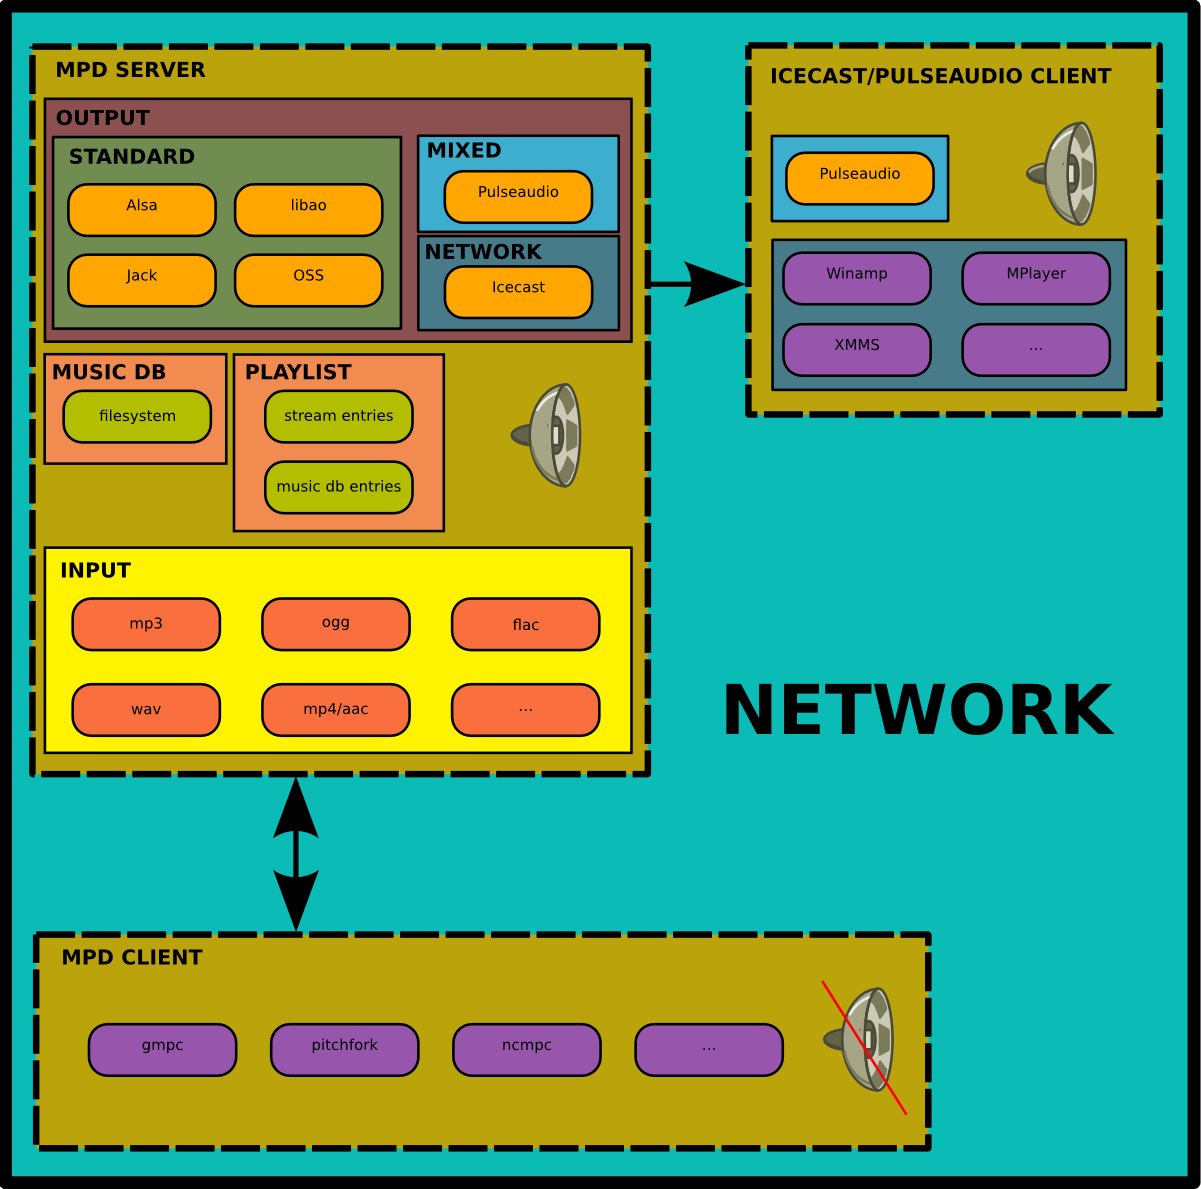
\includegraphics[scale=0.6]{./gfx/misc/Mpd-overview.png}
\end{figure}
\footnote{Bild-Quelle: http://images.wikia.com/mpd/images/6/68/Mpd-overview.png}
Der MPD-Server bekommt als Input mp3, ogg, flac, wav, mp4/aac,... Musik-Dateien die entweder in einer
Musik-Datenbank oder in Playlisten gespeichert sind. Der Standardoutput des MPD ist Alsa, libao, jack 
oder OSS, die Musik kann aber auch über einen Icecast oder Pulseaudio Clienten ausgegeben werden.
Der MPD-Client steuert den MPD-Server und hat selbst keinen Audio-Output.
